%!TEX root = main.tex


In this section, we empirically evaluate the effectiveness and the efficiency of the
state-of-arts in deep reinforcement learing on OpenAI gym Atari environment. Note 
that at current stage, we didn't propose any new methods in deep reinforcement learning;
instead our first stage is to learning the most advanced algorithms first using public
available online resources. 


\subsection{Environments}

In order to evaluate the algorithm, we conduct our experiments on Atari environment
provided by OpenAI. The description of Atari environment is as follows:
\begin{quote}
Maximize your score in the Atari 2600 game. In this
environment, the observation is an RGB image of the screen, which is an array
of shape (210, 160, 3) Each action is repeatedly performed for a duration of
kk frames, where kk is uniformly sampled from \{2, 3, 4\}~\cite{brockman2016openai}
\end{quote}

We choose three Atari games as our testing environment, all of which are unsolved environments, 
which means those games don't have a specific reward that you can consider it as the end of game:

\begin{enumerate}
\item Breakout-v0\\
In this game, player control a paddles at the bottom of screen and try to bounce the ball upwards
to hit those bricks as soon and as much as possible, as illustrated in Fig~\ref{fig:A3C_baselines} (a). 

\item Pong-v0\\
In this game, players control a paddles at the right of screen and try to bounce the ball pass the
other player at the left of screen, as illustrated in Fig~\ref{fig:A3C_baselines} (b). 

\item Phoenix-v0
In this game, players control a spaceship by moving it horizontally at the bottom of screen, as 
illustrated in Fig~\ref{fig:A3C_baselines} (c), trying to destroy the enemies by firing upwards 
and avoiding the attack from those enemies. 
\end{enumerate}

\subsection{Baselines}

In this section, we introduce the implementation details of the baselines we used.

% As we introduced in Methodology section, we use two neural network to model policy function
% and value function, respectively. 
The structure of policy network is shown as follows:
\begin{enumerate}
\item Convolution layer: $(5 \times 5, 32)$ 
\item Maximum pooling layer: $(2 \times 2) $
\item Convolution layer: $(5 \times 5, 32)$ 
\item Maximum pooling layer: $(2 \times 2) $
\item Convolution layer: $(4 \times 4, 64)$ 
\item Maximum pooling layer: $(2 \times 2) $
\item Convolution layer: $(3 \times 3, 64)$ 
\item Fully connected layer with 512 nodes and PReLU activation function.
\item Softmax layer to predict the probability over all possible actions.
\end{enumerate}
We modified the implementation of A3C from \href{https://github.com/ppwwyyxx/tensorpack}{tensorpack} repository.


\subsection{experimental results}
The experimental results are illustrated in the Fig~\ref{fig:A3C_baselines}. Please also
see the video animation by clicking the captions under each figures. 

\begin{figure}[h!]
\label{fig:A3C_baselines}
\centering
\begin{tabular}{c}
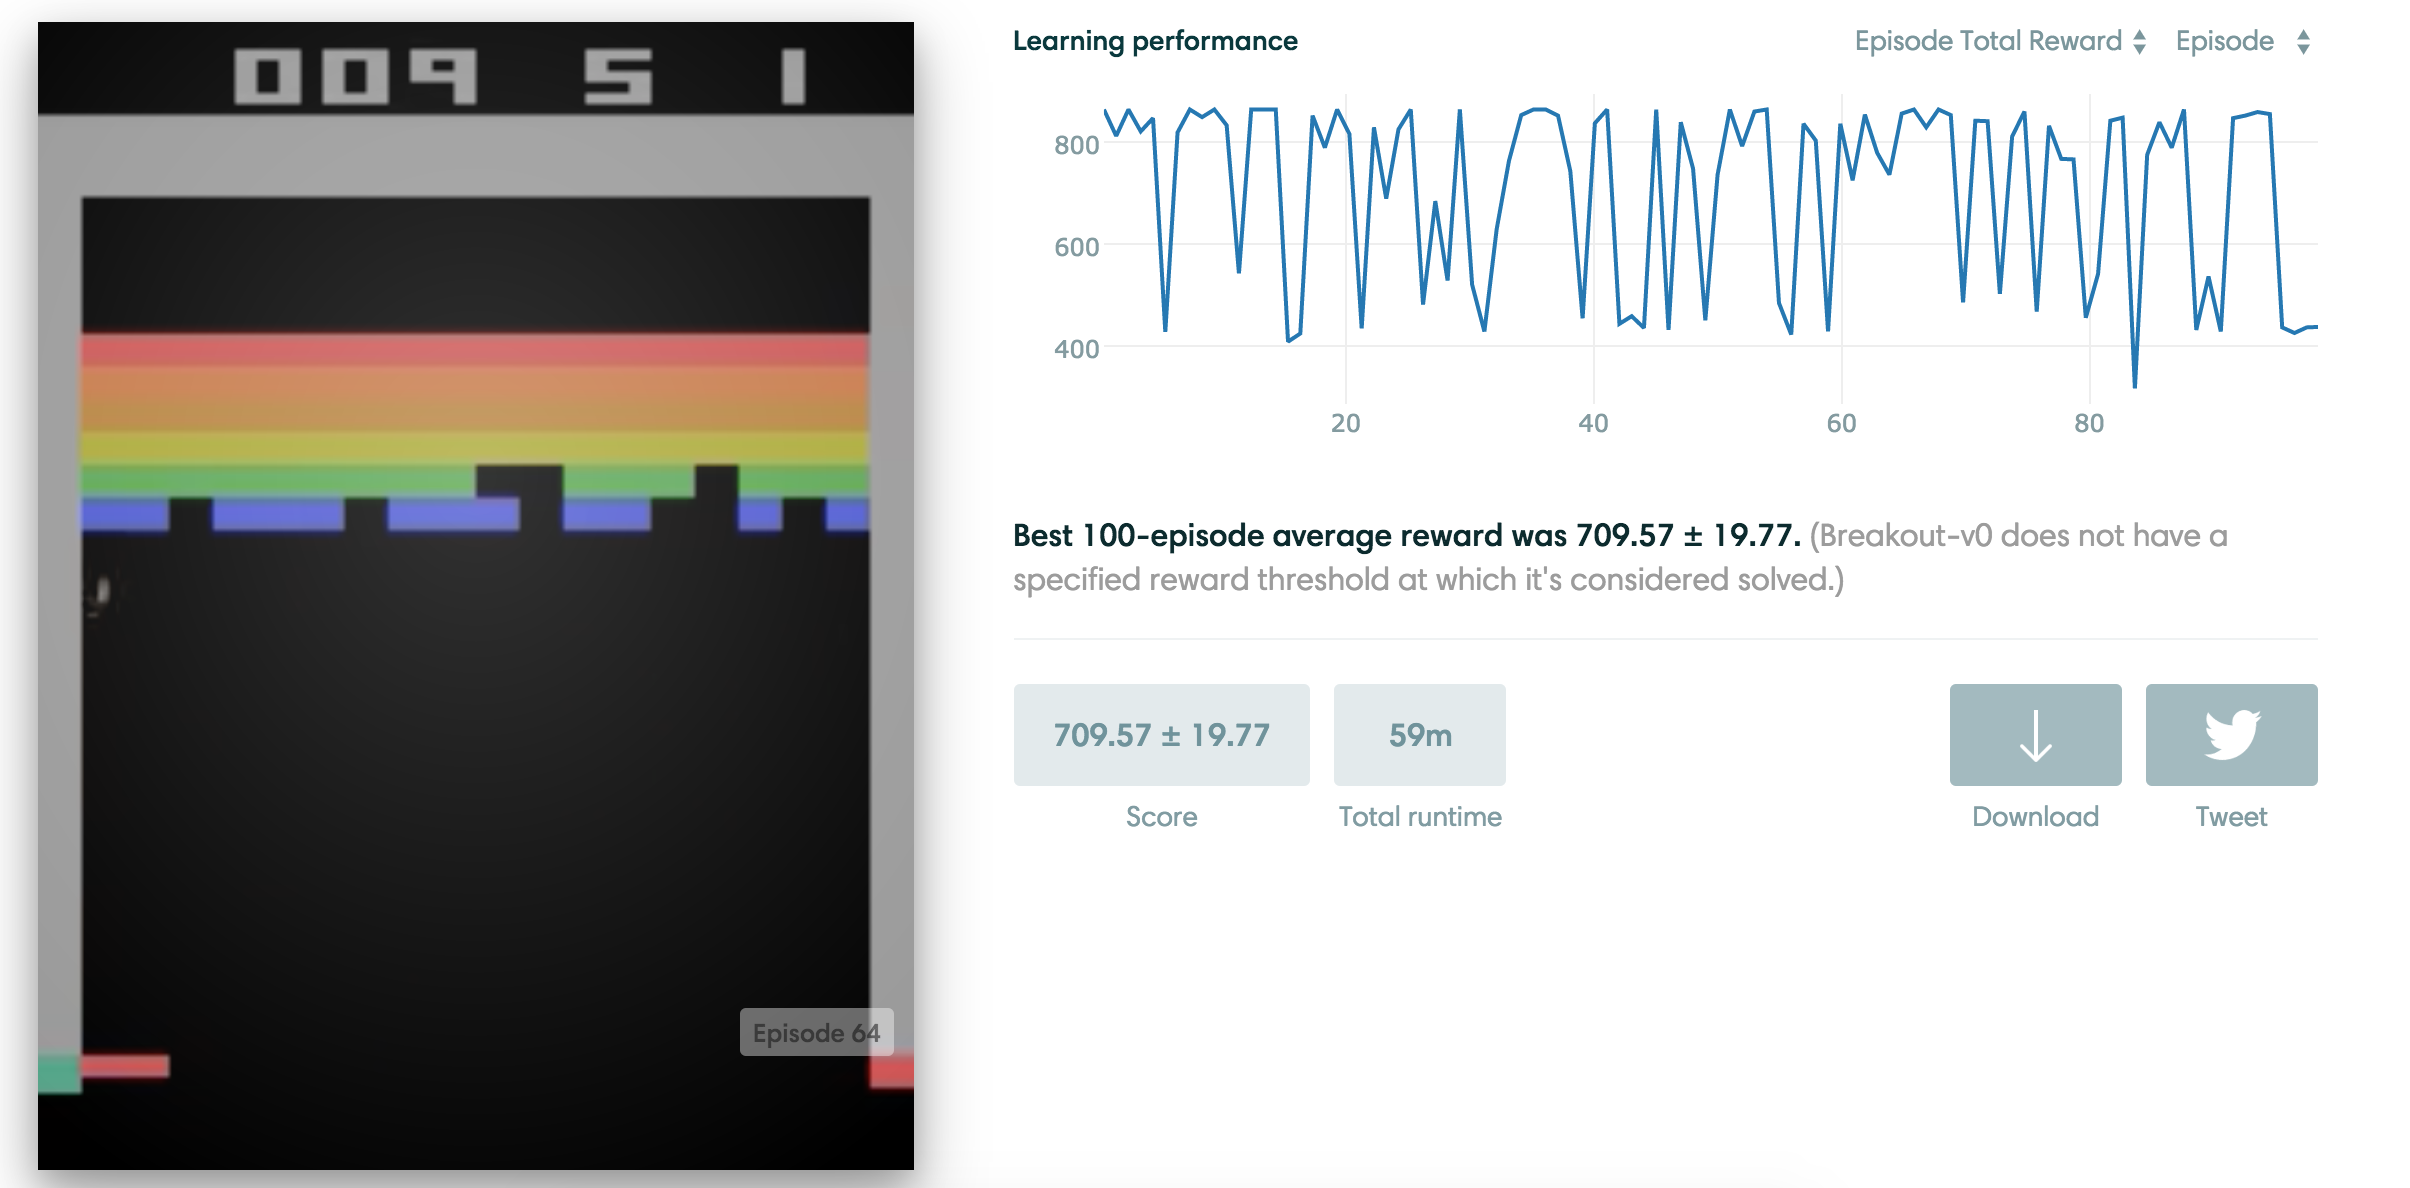
\includegraphics[width=0.49\textwidth]{./fig/A3C_Breakout-v0.png} \\
(a) \href{https://gym.openai.com/evaluations/eval_i9E40nAQuOTiSa0bxYBA#reproducibility}{Breakout-v0} \\
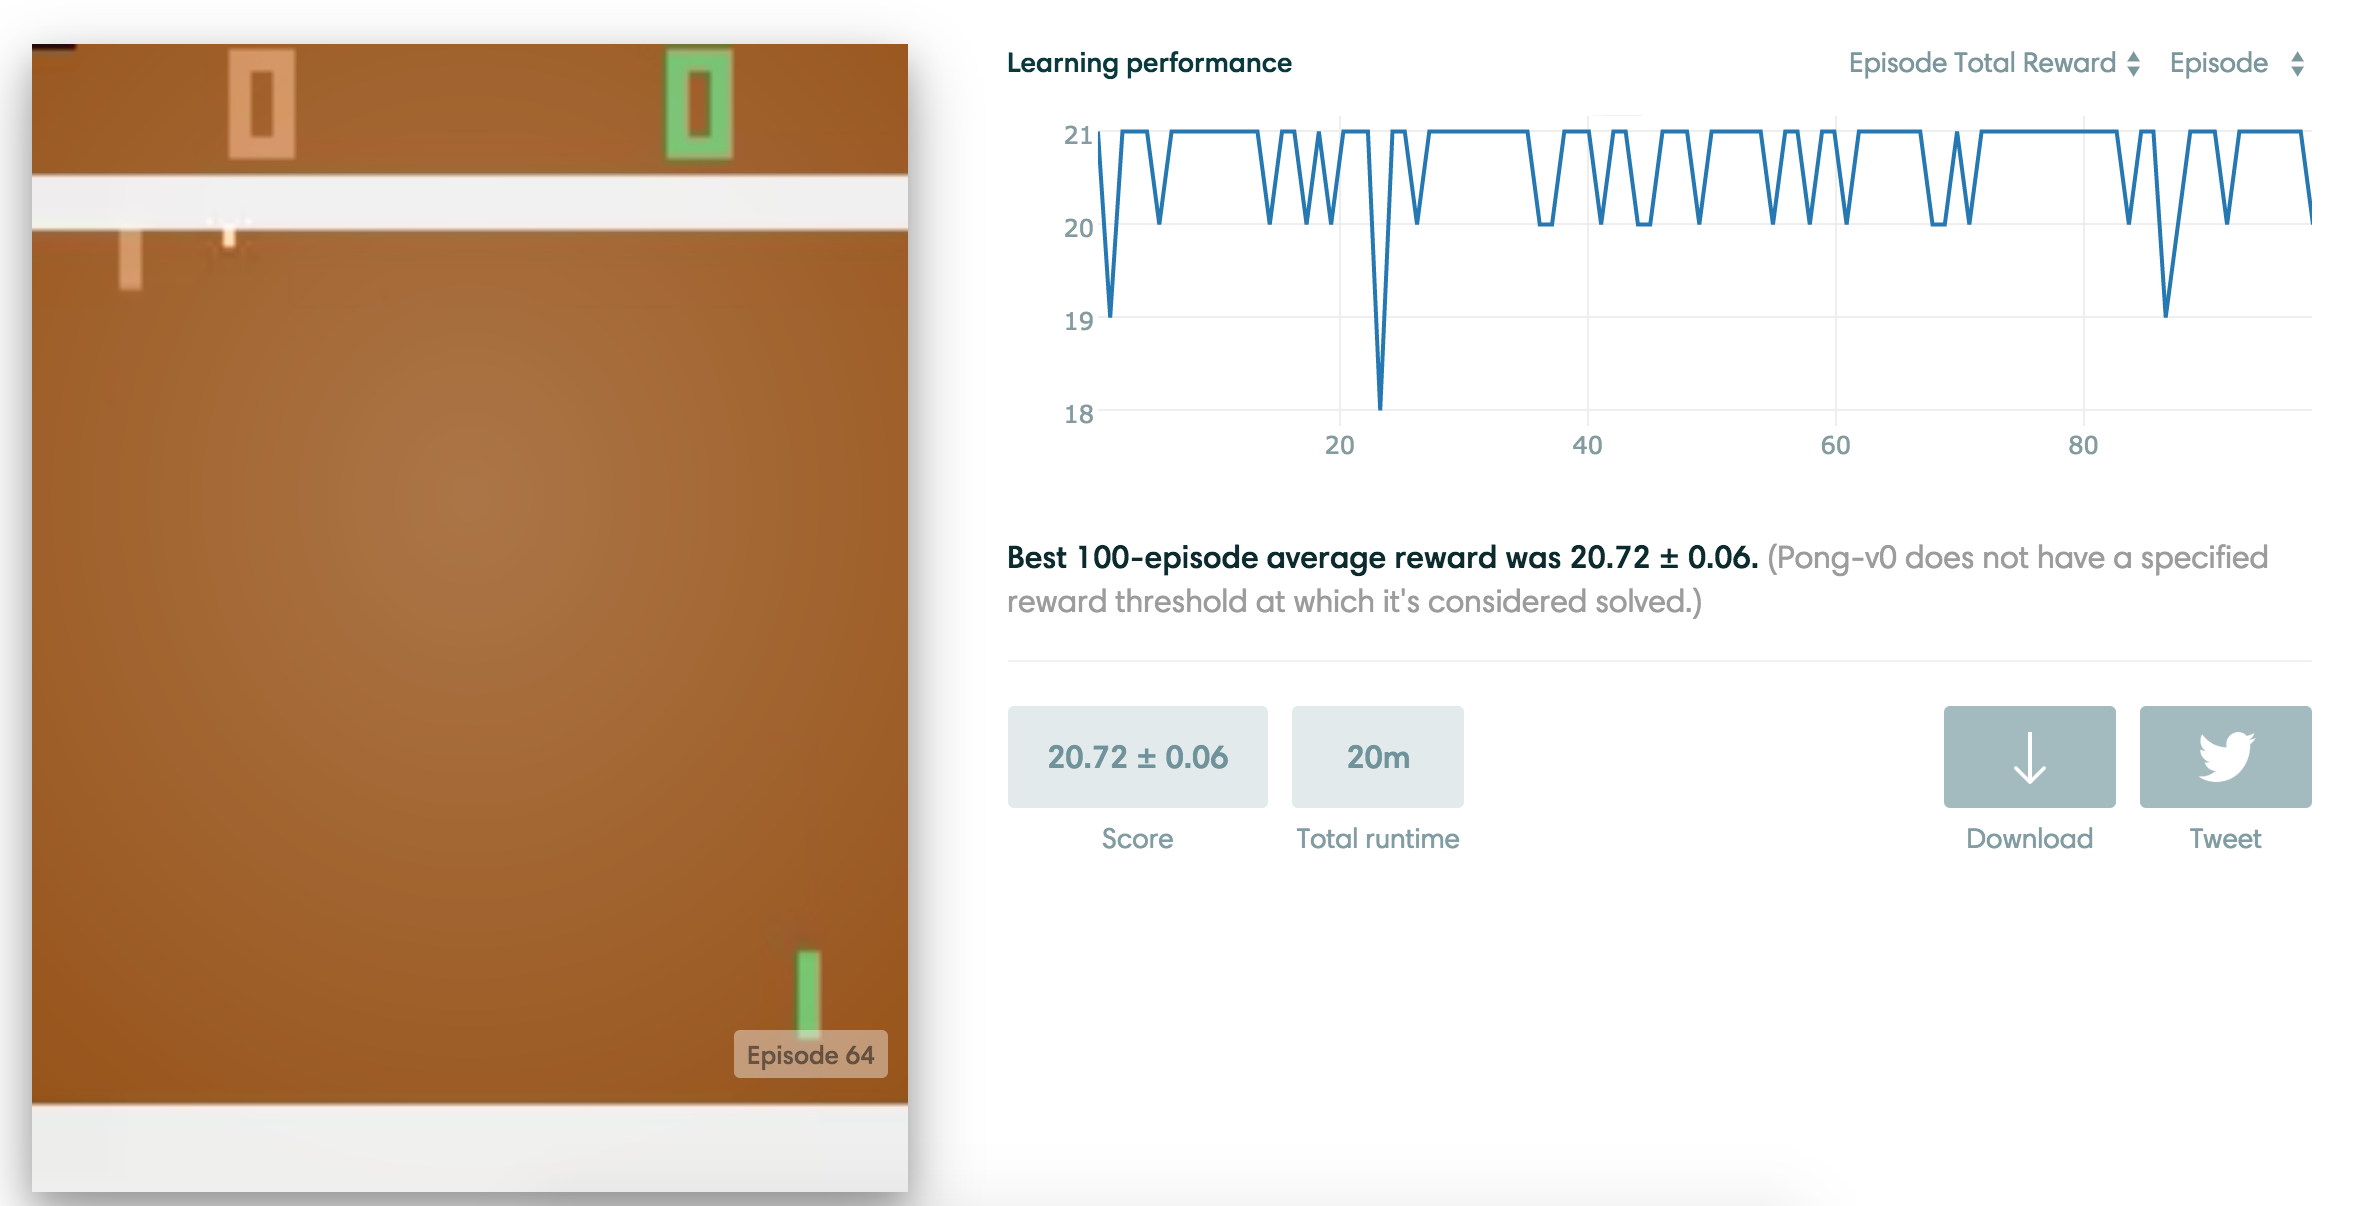
\includegraphics[width=0.49\textwidth]{./fig/A3C_Pong-v0.png} \\
(b) \href{https://gym.openai.com/evaluations/eval_mvXuxP13SSacO01UIhsg#reproducibility}{Pong-v0} \\
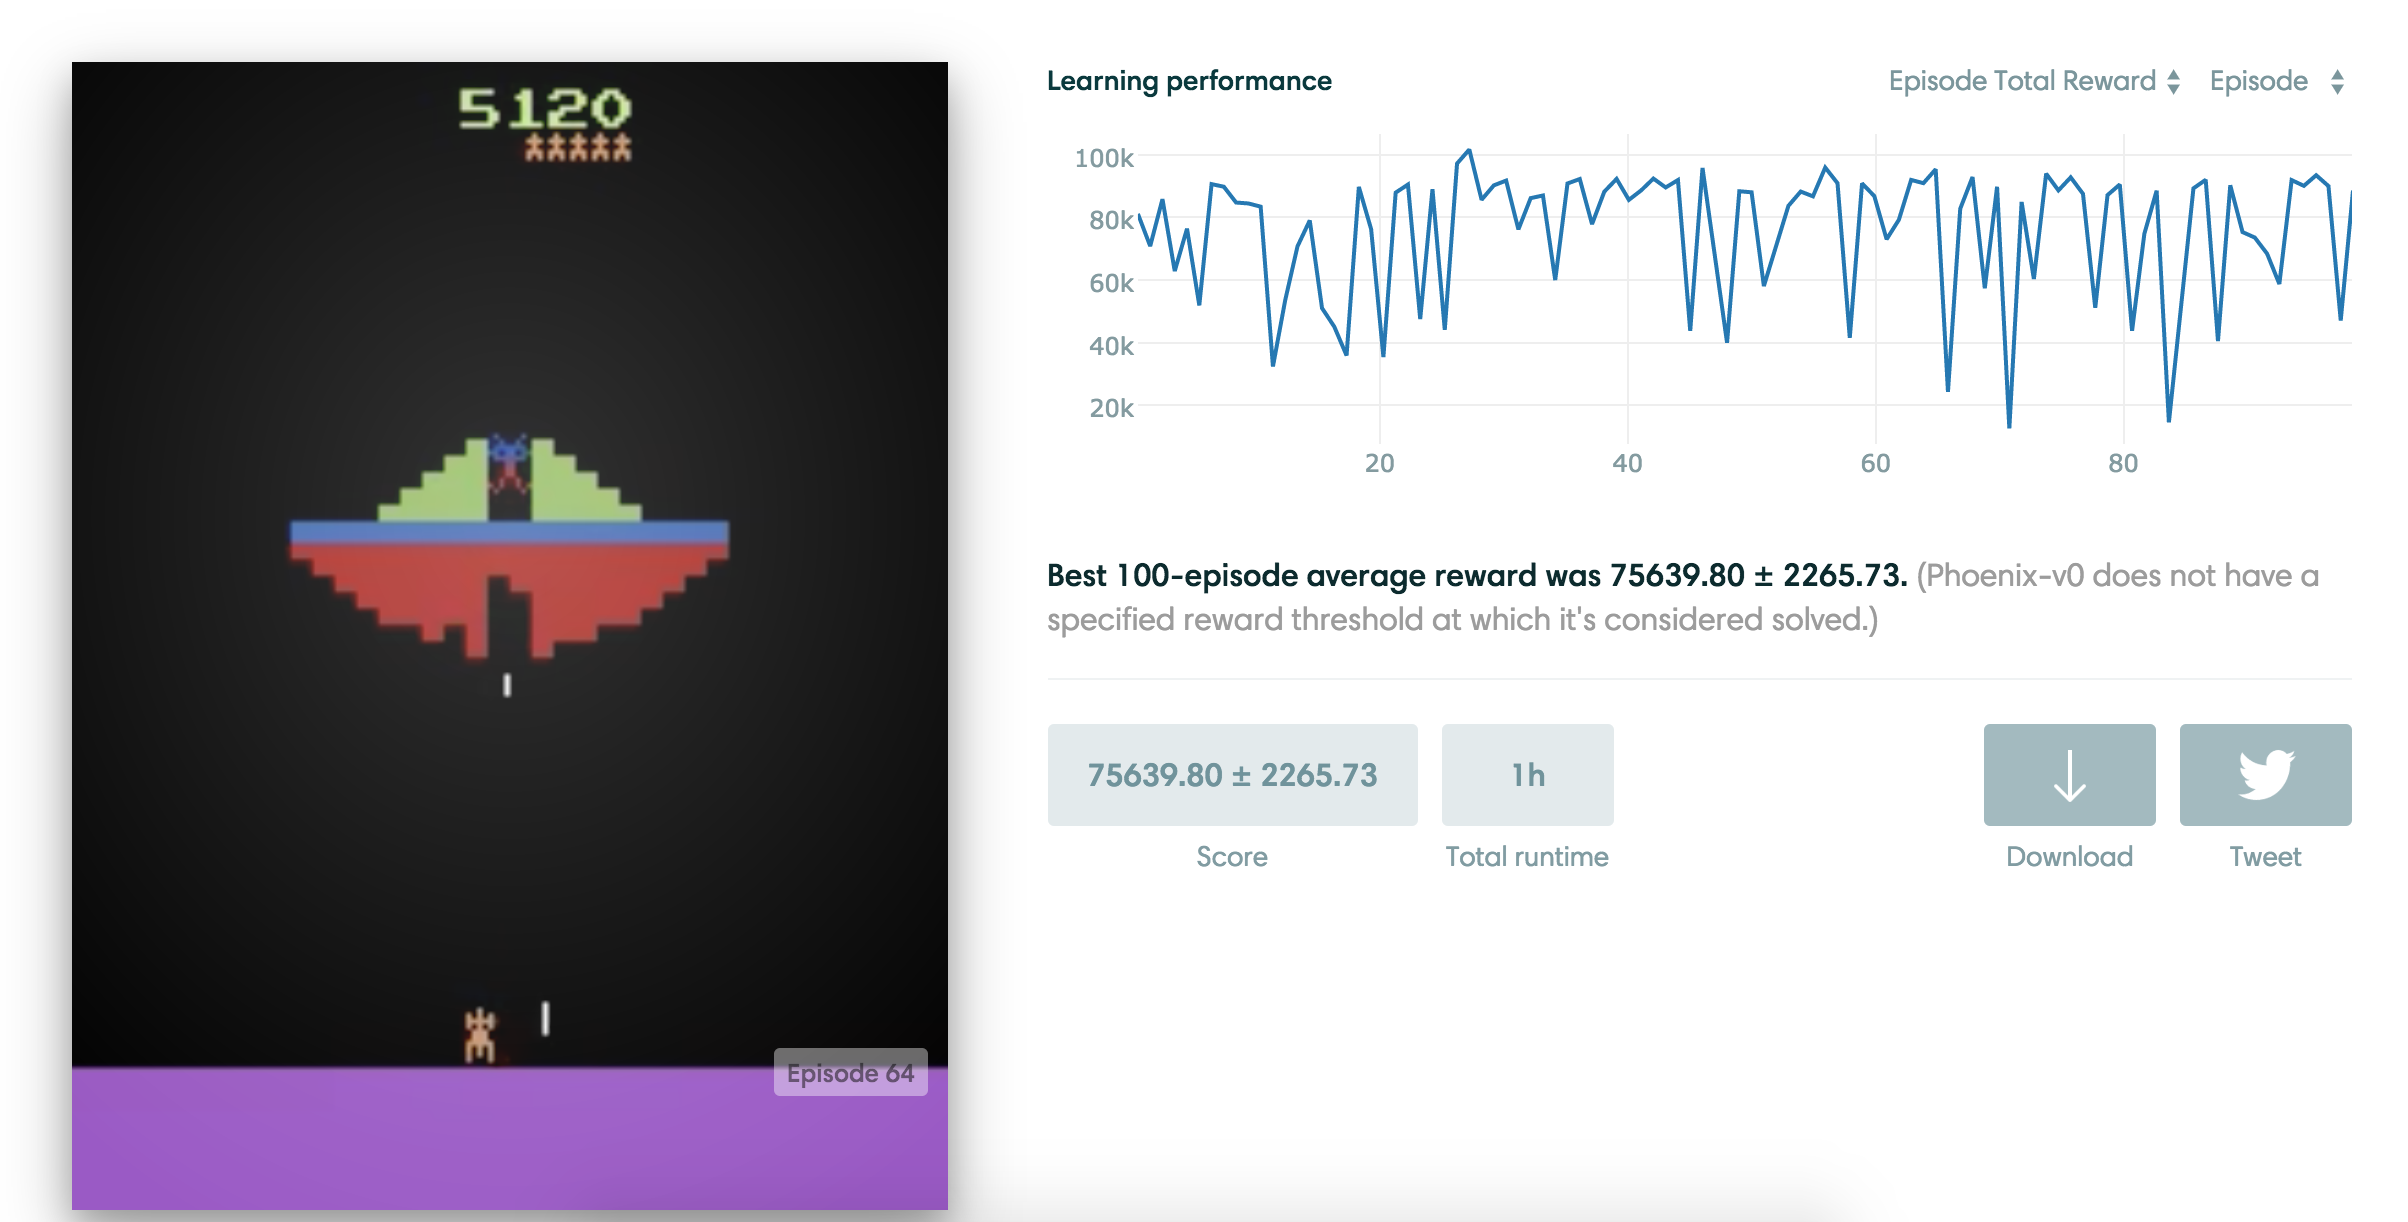
\includegraphics[width=0.49\textwidth]{./fig/A3C_Phoenix-v0.png} \\
(c) \href{https://gym.openai.com/evaluations/eval_Gva8XrEvTQi63KOd5Gyq1Q#reproducibility}{Phoenix-v0} \\
\end{tabular}
\caption{The results of 100 epsiodes on three environments by applying A3C algorithms. By clicking the name of each environment 
beneath the figures, you will see the video for each game played by trained agent.}
\end{figure}

